\chapter{Opis implementacije}
Implementacija uglavnom slijedi algoritam HERA \engl{Highly Efficient Repeat Assembly} opisan u radu \citep{Du345983} uz nekoliko manjih modifikacija. Algoritam se sastoji od tri glavnih koraka. Prvo se gradi graf preklapanja u kojem se traže putevi između contig-a. Nakon što su pronađeni mogući putevi, za svaki par contig-a se traži reprezentativna sekvenca te se u konačnici sastavlja jedna sekvenca između povezanih contig-a.

Alat Minimap2, ukoliko pronađe preklapanje između dvije sekvence (očitanje ili contig), da informacije o indeksima početka i kraja preklapanja za obje sekvence. Prvi korak je odbacivanje preklapanja koja zadovoljavaju barem jedan od sljedećih uvjeta:

\begin{itemize}
\item preklapanje je između dvije iste sekvence,
\item preklapanje u kojem jedna sekvenca u potpunosti sadrži drugu,
\item SI \engl{sequence identity} mjera je ispod određene granice (primjerice 40\%).
\end{itemize}

\begin{figure}[htb]
\centering
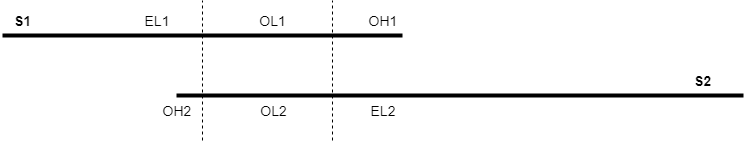
\includegraphics[width=\textwidth]{img/overlap.png}
\caption{Primjer preklapanja između S1 i S2}
\label{fig:overlap}
\end{figure}

Za preostale sekvence se računaju mjere preklapanja i produživanja. Na slici \ref{fig:overlap} je prikazano preklapanje između sekvenca $S_1$ i $S_2$ gdje se sekvenca $S_2$ nalazi nakon sekvence $S_1$. U sredini između isprekidanih linija je regija preklapanja čija je duljina $OL_1$ i $OL_2$, ovisno koju sekvencu gledamo, a izvana su $OH$ \engl{overhang length} i $EL$ \engl{extension length}. Koristeći navedene duljine, računa se mjera preklapanja $OS$ i mjere produživanja $ES_1$ i $ES_2$ prema izrazima \ref{eq:os} - \ref{eq:es2}. Pri tome je potrebno voditi računa preklapaju li se sekvence na istim ili suprotnim lancima. Primjerice da se $S_1$ i $S_2$ preklapaju na suprotnim lancima, potrebno bi bilo zamijeniti vrijednosti $OH_2$ i $EL_2$.

\begin{equation}
OS = \frac{(OL_1 + OL_2) * SI}{2}
\label{eq:os}
\end{equation}
\begin{equation}
ES_1 = OS + \frac{EL_1}{2} - \frac{OH_1 + OH_2}{2}
\label{eq:es1}
\end{equation}
\begin{equation}
ES_2 = OS + \frac{EL_2}{2} - \frac{OH_1 + OH_2}{2}
\label{eq:es2}
\end{equation}

Nakon što su sve mjere izračunate, odbacuju se preklapanja gdje je zbroj $OH_1$ i $OH_2$ veći od 20\% duljine produživanja $EL_1$ ili $EL_2$ te je moguće prijeći na izradu grafa preklapanja.

\section{Graf preklapanja}
Čvorovi u grafu predstavljaju contig-e i očitanja, a grane preklapanja, s time da grana može biti povezana na glavu ili rep čvora. Drugim riječima, svaki čvor ima svoje prefikse i sufikse. Sljedeći korak je traženje puteva između dva contig-a koji se obavlja pretraživanjem u dubinu \engl{DFS} uz nekoliko pravila. Postupak kreće iz svakog contig-a i zaustavlja se kada dođe do očitanja koje je povezano s drugim contig-om ili je trenutni put veći od maksimalne dopuštene duljine. Dodatno ograničenje je da se jedno očitanje ne može više puta pojaviti u istom putu.

Za izgradnju puteva koriste se tri pristupa. Prvi pristup iz početnog contiga izabere sve produžetke, ali za svaki sljedeći produžetak bira onaj koji ima najveću mjeru preklapanja $OS$. Ukoliko se dođe do čvora koji nema produžetke, vraća se jedan korak nazad i bira sljedeći najbolji produžetak. Drugi pristup radi isto kao prvi jedino koristi mjeru produživanja $ES$. Konačno, treći pristup nasumično bira produživanja proporcionalno mjeri produživanja $ES$, s time da je potrebno odrediti koliko puta će se iz svakog contig-a pokušati pronaći put ovom metodom. Po završteku postupka pronalaženja puteva između contig-a potrebno je samo odbaciti duplikate i moguće je prijeći na sljedeći korak algoritma.

\begin{figure}[htb]
\centering
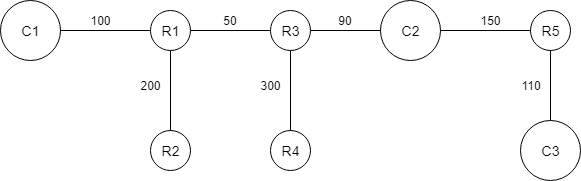
\includegraphics[width=\textwidth]{img/graph.png}
\caption{Primjer grafa preklapanja}
\label{fig:graph}
\end{figure}

Na slici \ref{fig:graph} je primjer jednostavnog grafa preklapanja gdje brojevi na granama predstavljaju mjeru preklapanja $OS$. Pretpostavimo da tražimo put iz contig-a $C_1$ prvim pristupom. Prvo ćemo produžiti put u $R_1$, nakon toga u $R_2$ jer ima veću mjeru preklapanja od puta koji vodi u $R_3$. Međutim, kako dalje nema čvorova moramo se vratiti nazad i ići u $R_3$. Iako je po mjeri preklapanja veći put u $R_4$, za sljedeći čvor biramo $C_2$ jer predstavlja contig i time je jedan put završen.

\section{Generiranje konsenzusa}
Jednom kada je konstruiran graf preklapanja, od potencijalno velikog broja pronađenih puteva između svakog od parova contig-a potrebno je odabrati jednu  reprezentativnu (konsenzusnu) sekvencu \engl{consensus sequence}.

Proces odabira takve sekvence započinje grupiranjem pronađenih puteva u tzv. konsenzusne grupe temeljem distribucije njihovih duljina, pri čemu razlikujemo 3 različita slučaja.

\begin{enumerate}
\item Prvi slučaj nastupa ukoliko su duljine svih pronađenih puteva usko distribuirane (unutar 10 kilobaza). Tada se svi putevi slažu u istu grupu, a kao reprezentativna sekvenca odabire se ona s najvećom prosječnom \textit{sequence identity} mjerom.

\item Ukoliko su duljine distribuirane šire od 10 kb, no ne šire od 100 kb, pokušava se formirati više konsenzusnih grupa. Na početku se putevi razvrstavaju (temeljem njihove duljine) u 10 podgrupa veličine 10 kb, koje pokrivaju čitavo područje distribucije. Zatim se za svaku podgrupu koja sadrži barem jedan put izračuna suma globalnih frekvencija pojavljivanja sadržanih puteva određene duljine. Sve podgrupe čija je suma frekvencija manja od $20\%$ najveće sume označavaju se kao doline \engl{valleys} dok u suprotnom postaju vrhovi \engl{peaks}. Nad tako označenim podgrupama tada se traže sve doline okružene s vrhovima te ukoliko iste postoje, duljina puta s najmanjom globalnom frekvencijom pojavljivanja svake od njih postaje granična duljina cijepanja glavne grupe (u kojoj su prvotno sadržani svi putevi). Pronalazak $n$ takvih dolina dovodi do cijepanja glavne grupe na $n + 1$ dijelova, od kojih svaki postaje zasebna konsenzusna grupa čija se reprezentativna sekvenca bira identično kao i u prvom slučaju.

\item Ukoliko su duljine distribuirane šire od 100 kb, u potpunosti se odbacuje mogućnost odabira reprezentativne sekvence između tog para contig-a.
\end{enumerate}
Nakon stvaranja svake od grupa, iz istih se filtriraju putevi čija je frekvencija pojavljivanja duljine manja od $50\%$ najveće frekvencije. Jednom kada su stvorene grupe između svih parova contig-a prelazi se na zadnji korak algoritma.

\section{Mihaela}